\chapter{Experiment with real users}

\label{ch:experiment}

	In spite of the efforts that have been made in order to approximate human-machine dialogue through simulation, there are still many complex behaviours and subtleties that could not be replicated. In this chapter the simulation results are tested with real users in a real dialogue setup as a validation (submitted as \cite{Khouzaimi2016b}). In the following, the interaction domain is presented then the experimental protocol is described. Finally, the result experiments are depicted and discussed.

\section{The Majordomo domain}

	The prototype used for the experiment (called Majordomo) has been implemented as a part of the VoiceHome\footnote{FUI project.} project at Orange Labs. This project is aimed at exploring the new opportunities that the use of the vocal modality to communicate with a smart home can bring. For that reason and in order to show that the methodology presented in this thesis is not domain dependent, this new task has been used for experiments instead of the agenda management task (event though they are somehow quite similar).
	
	Majordomo is able to schedule a set of tasks during a specific time window. These tasks are depicted in Table \ref{tab:majtasks}.

	\begin{table}[th]
	  \footnotesize
	  \centerline{
	  \begin{tabular}{|c|c|}
	      \hline
	      Task & Conflicting tasks \\
	      \hline
	      Alarm & Laundry, Hoover \\
              Heating & Open windows, Air conditioning \\
              Open windows & Heating, Air conditioning \\
              Absence mode & Open windows \\
              Laundry & Alarm, Calm mode \\
              Air conditioning & Heating, Open windows \\
              Swimming pool warming & Swimming pool cleaning \\
              Swimming pool cleaning & Swimming pool warming \\
              Calm mode & Laundry, Hoover, Mow lawn \\
              Mow lawn & Water lawn \\
              Water lawn & Mow lawn \\
              Record channel 1 & Record channel 2, Record channel 3 \\
              Record channel 2 & Record channel 1, Record channel 3 \\
              Record channel 3 & Record channel 1, Record channel 2 \\
              Hoover & Alarm, Calm mode \\
              Run bath & \\
	      \hline
	  \end{tabular}
	  }
	  \caption{Majordomo tasks}
	  \label{tab:majtasks}
        \end{table}

	However some tasks cannot be run simultaneously (in Table \ref{tab:majtasks}, the second column shows which tasks cannot be scheduled at the same time as the one in the first column). For example:
	
	\begin{itemize}
		\item The lawn cannot be mowed while watered.
		\item The heating cannot be activated when the windows are open.
		\item The swimming pool cannot be warmed and cleaned at the same time.
		\item When the calm mode is activated, no hoovering nor laundry are allowed.
	\end{itemize}
	
	This is a slot-filling task where the user is supposed to provide the following information: the action type (ADD, MODIFY or DELETE), the task (see the list above), the date and the time window.

\section{Experimental protocol}

	\subsection{Implementation}
	
		The Client (interface to the users) has been developed in the form of a website where the users are supposed to read a few instructions before starting to interact with the system. Google ASR has been chosen since it is a powerful off-the-shelf solution that does not require to develop any acoustic nor language model, which is costly and not in the focus of this work. It also has a powerful named entity recognition engine (NER, see \cite{BenJannet2015}) and it is able to provide incremental partial results. However, it is still not able to provide the partial confidence scores (only the confidence score at the end of the utterance is computed).
		
		The implementation of the Service is similar to the personal agenda management case described in the previous chapters. The only difference is that home tasks are manipulated instead of events. Therefore, an open slot has been replaced with a slot where only a few alternatives are possible. Moreover, in the personal agenda management domain, no events can overlap whereas in the Majordomo domain some tasks can be run at the same time as others and others cannot. This is encoded in a compatibility matrix provided to the Service.
		
		As far as the Scheduler is concerned, similarly to the strategies developed in the simulation case, a handcrafted (version presented in Chapter \ref{ch:baseline}, with no FEEDBACK\_RAW) as well as a reinforcement learning strategy have been implemented. The reinforcement learning strategy has been learnt in simulation (the US has also been ported to the new domain) and tested directly with real users. Since Google ASR does not provide the confidence scores incrementally, this feature has been removed from the model. Finally, when transitioning from simulation to the real word, there is no need to estimate timing from the number of words, therefore, real timestamps have been taken into account.
		
	\subsection{Conduct of the dialogue}
	
		Once the user decides to start a dialogue, the system displays the interface depicted in Figure \ref{fig:majordomo}. A small briefing paragraph explains the task to accomplish which is also synthesised in the form of a table. Ten different scenarios were designed and one of them was picked randomly at each new interaction. Similarly, the dialogue strategy is also picked randomly: the user can interact with the non-incremental strategy, with the handcrafted incremental or the reinforcement learning incremental strategy, but she is not aware which one is used for each dialogue.
		
		When ready, the user clicks on the \textit{Start} button. During the interaction, the ASR is always on so the Client is always listening except in the system barges-in, in which case it is disabled for two seconds. This is necessary in order to make the system take the floor, otherwise, it will be immediately interrupted before the user even realises that there is an intervention.
		
		After the interaction, either the user ends the dialogue normally by saying \textit{Goodbye} or hangs up by clicking on the \textit{Hang up} button.
	
	\begin{figure*}[htp]
		\centering
%		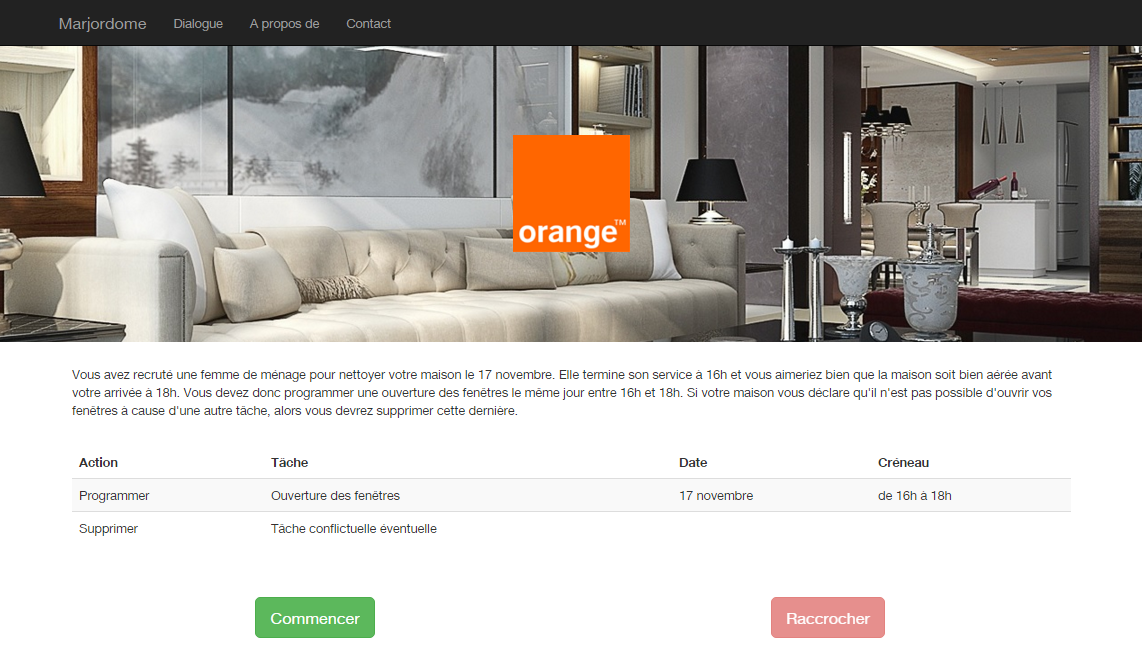
\includegraphics[scale=0.48]{figures/majordome.png}
                \rotatebox{90}{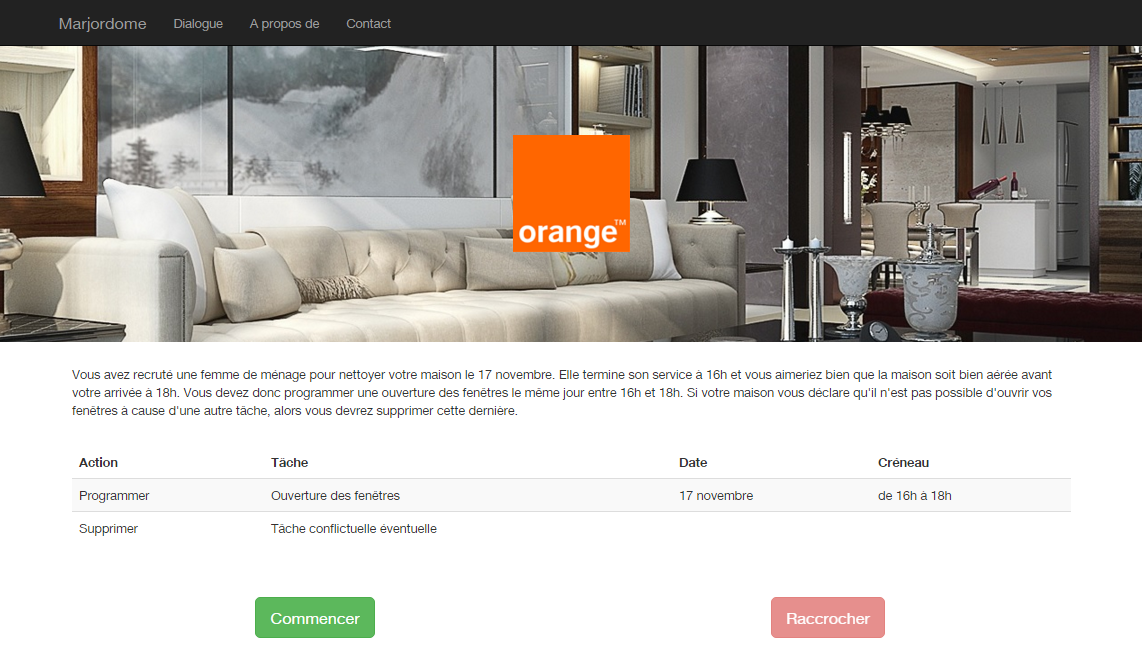
\includegraphics[scale=0.65]{figures/majordome.png}}
		\caption{The Majordomo interface}
		\label{fig:majordomo}
	\end{figure*}
	
	\subsection{Key Performance Indicators}
	
		In order to evaluate the three turn-taking strategies, dialogue duration and task completion have been computed (the tasks scheduled by the Majordomo are logged at the end of the dialogue). In addition, the users filled a survey at the end of each dialogue where they provided the following subjective Key Performance Indicators (KPIs) on Lickert scales:
		
		\begin{itemize}
			\item \textbf{Reactivity:} The users are asked whether they found the system reactive or not. There are 6 possible answers going from 1 (\textit{not reactive at all, very slow}) to 6 (\textit{very reactive}).
			\item \textbf{Reactivity impact:} The system's reactivity does not necessarily improve the dialogue quality since it can be perceived as too intrusive. The objective of this metric is to assess the impact associated with the reactivity through 6 possible values going from 1 (\textit{very negative, hurts the dialogue quality}) to 6 (\textit{very positive, significant improvement of the dialogue quality}).
			\item \textbf{Realism:} The users are asked whether the system acts like a human operator. There are 6 possible answers going from 1 (\textit{no, not at all}) to 6 (\textit{yes, clearly}).
			\item \textbf{Efficiency:} The users are asked to assess the dialogue efficiency by selecting one of the 6 possible answers, going from 1 (\textit{very bad}) to 6 (\textit{very good}).
			\item \textbf{Global quality:} The users are asked how they globally appreciated the dialogue on a scale from 1 (\textit{Very unpleasant experience}) to 6 (\textit{Very enjoyable experience}).
			\item \textbf{Potential user:} Finally, the users are also asked whether they would use the Majordomo at home (if it was a real commercialised product) on a scale from 1 (\textit{clearly not}) to 4 (\textit{absolutely}).
		\end{itemize}


\section{Results and discussion}

	206 dialogues have been collected with the collaboration of 47 volunteer users (from Orange Labs, LIA and personal network). 65 dialogues were run using the non-incremental strategy (\textit{None}), 65 using the handcrafted strategy (\textit{Handcrafted}) and 76 using the reinforcement learning one (\textit{RL}). The experiment results are depicted in Table \ref{tab:globalmetrics}.

	\begin{table}[th]
	  \footnotesize
	  \vspace{2mm}
	  \centerline{
	  \begin{tabular}{|c|c|c|c|c|}
	      \hline
	      Category & KPI & \textit{None} & \textit{Handcrafted} & \textit{RL} \\
	      \hline
	      \multirow{2}{*}{Objective} & Duration (sec) & 94.7 & \textbf{89.6} & 90.6 \\
	      & Task completion & 0.60 & 0.63 & \textbf{0.75} \\
	      \hline
	      \multirow{6}{*}{Subjective} & Reactivity & 4.31 & 4.57 & \textbf{4.62} \\
	      & Reactivity quality & \textbf{4.38} & 4.25 & 4.36 \\
	      & Human-likeness & 3.63 & 3.66 & \textbf{3.74} \\
	      & Efficiency & 4.22 & 4.20 & \textbf{4.36} \\
	      & Global quality & 4.06 & 4.18 & \textbf{4.20} \\
	      & Potential use & 2.66 & 2.68 & \textbf{2.82} \\
	      \hline
	  \end{tabular}
	  }
	  \caption{Global dialogue evaluation metrics}
	  \label{tab:globalmetrics}
        \end{table}

        As far as the mean dialogue duration is concerned, the incremental strategies slightly improve the dialogue duration (even though this is not statistically significant). At a first glance, this improvement can be viewed as an obvious result since by construction, incremental strategies are more reactive. Nevertheless, the user can also be interrupted before she has provided all the information that she wanted which complicates the dialogue and makes it last longer like it is the case in the experiment led in \cite{Ghigi2014}. Therefore, this result shows that the Majordomo successfully interrupted the user on average. However, there is no visible change when comparing the \textit{Handcrafted} and the \textit{RL} strategy.

        The task completion ratio, on the other hand, has been significantly\footnote{All the p-values are computed according to the Welch t-test since the number of samples is important enough for the means to be considered as following a normal distribution (and since it is more powerful than non-parametric tests). A binomial proportions test has also been run for task completion, leading to very similar p-values.} improved by the \textit{RL} strategy compared to \textit{None} (by 15\% with $p = 0.030$). Moreover, an important difference has been reported between \textit{RL} and \textit{Handcrafted} (12\%) even though it is not exactly statistically significant ($p = 0.065$). Finally, \textit{Handcrafted} shows a minor improvement over \textit{None} (3\%) with no statistical significance ($p = 0.36$). The Majordomo task requires a certain level of engagement and focus in order to keep track of all what has been accomplished so far, while keeping the final objective in mind. When interacting with a reactive system that takes the floor in an intelligent way (to correct errors hence fixing desynchronisations, to deliver a response when all the information has been provided...) without overwhelming the user, the latter feels more engaged in the conversation thus accomplishing the task more efficiently, even when a certain cognitive load is involved. Another impact of such strategy as reported in \cite{Ghigi2014} is that when the users realise that they can be interrupted in case of a problem, they tend to provide more concise and focused answers, which reduces the risk of a misunderstanding.

        The subjective metrics are the noisier ones. Therefore, except from the \textit{Reactivity} KPI where \textit{RL} significantly improves it in comparison with \textit{None} ($p = 0.048$), the other p-values are above 0.05. Nevertheless, generally speaking, the metrics tend to favour the \textit{RL} strategy.

	\begin{table}[th]
	  \footnotesize
	  \vspace{2mm}
	  \centerline{
	  \begin{tabular}{|c|c|c|c|}
	      \hline
	      KPI & \textit{None} & \textit{Handcrafted} & \textit{RL} \\
	      \hline
	      Latency (ms) & 1545 $\pm$ 61 & 1303 $\pm$ 78 & \textbf{588 $\pm$ 59} \\
	      FC ratio & No barge-in & 0.31 $\pm$ 0.091 & \textbf{0.068 $\pm$ 0.023} \\
	      \hline
	  \end{tabular}
	  }
	  \caption{Local dialogue evaluation metrics}
	  \label{tab:localmetrics}
	\end{table}

        To complete this study, more local metrics have been investigated: the latency and the false cut-in ratio. The latency is the mean delay involved in each human to machine floor transition\footnote{Estimated as the delay between the moment when the Scheduler delivers the last message and the moment when it received the last ASR output. Computing the real latency requires a Voice Activity Detection (VAD) module in the Client which could slow it down.} (549 transitions for \textit{None}, 542 for \textit{Handcrafted} and 727 for \textit{RL}) whereas the false cut-in ratio refers to the proportion over all the SPEAK decisions (\textit{Handcrafted} : 99, \textit{RL} : 456) of the ones where the system should have waited longer before taking the floor (manually annotated). The results are reported in Table \ref{tab:localmetrics} (all the differences are statistically significant with $p < 0.000001$). The \textit{Handcrafted} strategy reduces the latency by 200ms compared to \textit{None}, however, it interrupts the user too soon one third of the time thus being too aggressive. On the other hand, \textit{RL} reduces the latency by 1 second while maintaining a more reasonable false cut-in ratio. As a consequence, \textit{RL} takes more risk since it chooses to SPEAK more often and when it does, it is better managed (significantly less frequent false cut-ins).

\section{Discussion}

        In comparison with previous work (see Chapters \ref{ch:soadialogue} and \ref{ch:soarl}), this is the first direct application of reinforcement learning to turn-taking management in an incremental dialogue system that is evaluated in real conditions. In many previous studies, an indirect way of testing dialogue strategies is used: controlled dialogue acts \cite{Aist2007}, a posteriori evaluation using recordings of interactions \cite{Meena2013}, a posteriori comparison with human decision corpus \cite{Jonsdottir2008,Dethlefs2012}, etc... As it is said in \cite{Aist2007}, the objective is \textit{to minimize variance due to extraneous factors such as interspeaker variability, acoustic noise, and so forth and concentrate specifically on the difference between incremental processing and its nonincremental counterpart}. However, the price to pay to reduce variance is a certain bias due to the fact that the experiment is not run in real conditions.

        Some papers use handcrafted strategies \cite{Raux2009,Ghigi2014}, some collect annotated corpora on which they run supervised learning algorithms \cite{Meena2013} and others propose reinforcement learning based strategies \cite{Jonsdottir2008,Selfridge2010,Dethlefs2012}. However, to our knowledge, live studies only fit in the first two categories and no purely autonomous system using reinforcement learning has been tested with real users and directly evaluated by them, in real dialogue conditions. More generally, previous work related to incremental dialogue processing and turn-taking optimisation can be split into two categories given the metrics that are involved:

        \begin{itemize}
          \item \textbf{Local metrics:} These studies are based on the principle introduced in \cite{Sacks1974} and saying that gaps and overlaps should be minimised in order to achieve smooth turn-taking. As a consequence, local metrics where only floor transitions are considered are used, mainly the latency and the false cut-in ratio \cite{Jonsdottir2008,Raux2012}.
          \item \textbf{Global metrics:} Considering the overall dialogue quality can also be a way of evaluating turn-taking strategies \cite{Selfridge2010,Ghigi2014}. Such an approach has the advantage of not having to make any assumption about what would make the dialogue more appealing for the user. However, the metrics involved are more difficult to measure since they are noisier.
        \end{itemize}

        In this thesis, global metrics were used for training then both global and local metrics were evaluated. Interestingly, it is shown that by optimising global KPIs, local ones turn out to be improved as well. Finally, even though it has been shown that interrupting the user can hurt its opinion on the system in some cases \cite{Hirasawa1999}, the results described above show that when it is done at the right moment, the system is stignificantly more efficient while being judged slightly better from a subjective point of view.

